\documentclass{article}
\usepackage[table,x11names,dvipsnames,table]{xcolor}
\usepackage{comment}
\usepackage{graphicx}
\graphicspath{ {./Images/} }

\usepackage{float}
\usepackage{hyperref}

\title{Het medisch vaststellen van de ABCDE lijst met een Arduino Due \thanks{Opdracht van de Hogeschool Utrecht voor het project R2D2 2019-2020}}
\author{Oscar Kromhout en Vincent van Setten\\ Team 3}

\date{April, 2020}


\begin{document}

\begin{titlepage}
	\centering
	\maketitle
	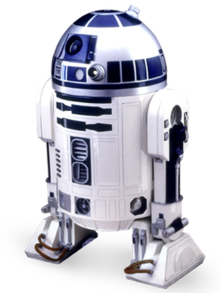
\includegraphics[scale=2.0]{title.png}
	\clearpage
\end{titlepage}

\tableofcontents
\clearpage 
\section{Samenvatting}
Hierin worden het onderzoek samengevat. Hier moeten sowieso de conclusies en resultaten in voor komen. De samenvatting moet onafhankelijk te lezen zijn en is bedoeld om een globaal overzicht te bieden.

\section{Voorwoord}
Dit onderzoek wordt gedaan voor het schoolproject R2D2 2020 in opdracht van de Hogeschool Utrecht. Hiervoor willen wij Diederik Yamamoto-Roijers bedanken voor zijn hulp in het ons leren onderzoek te doen en bedanken wij alle leden van Team 3: 
\begin{itemize}
	\item Niels Post
	\item Otto de Visser
	\item Amrit Malhi
	\item Menno van der Jagt
	\item Youri de Vor
	\item Finn Fonteijn
	\item Vincent van Setten 
	\item Oscar Kromhout
\end{itemize}

Verder willen wij de hogeschool Utrecht bedanken voor de opdracht en iedere docent die iets te maken heeft gehad met R2D2.

\begin{itemize}
	\item Jorn Bunk
	\item Diederik Yamamoto-Roijers 
	\item Hans Middelkoop
	\item Brian van der Bijl 
	\item Walter Willems 
	\item Wouter van Ooijen
\end{itemize}

Dit deelonderzoek is gedaan door Oscar Kromhout en Vincent van Setten.

\section{Inleiding}
De hoofdvraag van ons onderzoek gaat over het afwerken van de medische A.B.C.D.E. lijst. Met deze lijst bepalen medici in wat voor medische noodsituatie iemand verkeerd, en kan worden bepaald hoeveel hulp iemand nodig heeft. Om deze hoofdvraag te beantwoorden hebben wij ons onderzoek weer opgedeeld in een drietal kleinere deelonderzoeken.  
Een aantal van de onderdelen van de A.B.C.D.E lijst kunnen worden gecontroleerd met sensoren. Denk hierbij aan temperatuur, hartslag of zuurstofsaturatie. Maar bij een deel is dit lastig met sensoren op te lossen en is het verstandig daar een menselijk oog aan te pas te laten komen. Het is dus handig als medisch personeel op afstand zou kunnen (mee)kijken via een robot om iemands medische staat te controleren. Hiervoor willen wij deelonderzoek gaan uitvoeren naar de mogelijkheid een Arduino Due te gebruiken in combinatie met een camera. Om de scope van ons onderzoek te verkleinen doen we geen onderzoek naar het versturen van deze beelddata, maar wel naar het bufferen van deze beelddata zodat het in de toekomst verstuurd zou kunnen worden. 
Uit deze context hebben wij de volgende hoofdvraag afgeleid: 

\textit{Welke camera, compatibel met de Arduino due en onder de 28 euro, is het meest geschikt om de toestand van een patiënt te fotograferen of filmen en dit zo vlot en accuraat mogelijk lokaal te bufferen op het RAM geheugen van de Arduino due om wanneer het gebufferd kan worden, door te kunnen sturen naar medisch personeel voor de medische vaststelling van de A en D van de ABCDE lijst?}

Om deze hoofdvraag te beantwoorden hebben wij deze onderverdeeld in 8 deelvragen. Deze vragen lopen we systematisch en volgordelijk af om op die manier tot een antwoord op de hoofdvraag te komen. De deelvragen luiden als volgt:

\begin{enumerate}
	\item Bestaan er camera’s op de markt die geschikt zijn voor de Arduino Due, maar onder de 28 euro zijn?
	\item Welke factoren beïnvloeden welke camera het meest geschikt is voor onze toepassing? 
	\item Als er camera’s bestaan die aan onze geschiktheidseisen voldoen, welke zou dan het meest geschikt zijn voor deze toepassing? 
	\item Heeft de Arduino Due genoeg intern geheugen om één frame te bufferen met de meest geschikte camera? 
	\item Wat is het maximale aantal frames (of deel van een frame) dat wij met de gekozen camera kunnen bufferen op het RAM geheugen van de Arduino Due? 
	\item Kan alles van de A {\&} D van de ABCDE lijst gecontroleerd worden met een foto of filmpje? 
	\item Wat moet medisch personeel zien op een filmpje of foto om erachter te komen wat er medisch nodig is voor de A {\&} D van de ABCDE lijst? 
	\item Hoeveel frames moeten we bufferen om het voor medici mogelijk te maken, zover het mogelijk is via beelden, de A {\&} D controle te doen? 
\end{enumerate}
De precieze uitwerking van deze deelvragen wordt beschreven in het hoofdstuk “Opzet en Uitvoering van het onderzoek”.
De doelgroep van ons onderzoek zijn tweedejaars technisch informatica studenten. Dit onderzoek moet immers weer opnieuw worden gebruikt in de hierop volgende jaren tijdens het R2D2 project.

\begin{comment}
Hier moeten nog 2 referenties naar de research papers!
\end{comment}

\section{Literatuurverkenning}
We hebben twee relevante research documenten gevonden.
De eerste hiervan is “Surveillance Robot Using Arduino Microcontroller, Android APIs and the Internet”. In dit onderzoek wilden men een live video feed gebruiken voor een surveillance robot. In dit onderzoek gebruikten ze een android telefoon om de video feed te realiseren(het was gewoon een telefoon verbonden met een robot). 
Het tweede onderzoek is genaamd “Spy Robot Wireless Video Surveillance using Arduino”. 
In dit onderzoek willen ze ook een live feed opstellen. In dit onderzoek was het doel om een robot te maken die op afstand kon surveilleren, zodat hier geen mensen op het spel worden gezet in, bijvoorbeeld, een oorlog op het terrein van de vijand. 
In dit onderzoek hebben ze deze video feed gerealiseerd met een IP-camera, die zelf de beelden verstuurd via wifi. 
Deze onderzoeken hadden hetzelfde uiteindelijke doel, namelijk het realiseren van een live video feed door middel van een Arduino Due. Helaas hebben we weinig gehad aan deze onderzoeken, omdat zij oplossingen gebruiken die niet bruikbaar zijn in ons onderzoek. Zij gebruiken een mobiele telefoon en een IP camera. Een mobiele telefoon is iets wat wij niet willen gaan doen, omdat wij onze robots modulair willen hebben. Een telefoon vastknopen aan een robot is niet erg handig. Daarnaast is het ook erg duur. Dat laatste geldt ook voor de IP camera. Het is een stuk duurder dan een gebruikelijke Arduino camera.
Behalve deze twee literatuur stukken hebben we niet heel veel kunnen vinden dat iets te maken had met ons onderzoek. 

\section{Probleemstelling}
Filmen met een camera, deze data verwerken en deze data opslaan zijn zware taken voor een computer. We hebben een camera nodig die het mogelijk maakt met een Arduino Due foto’s te maken. Deze beelden moeten van voldoende kwaliteit en kwantiteit voor medisch personeel zijn. Als we in staat zijn om met een camera geschikte beelden te maken met een Arduino Due, moeten we die beelden ook nog kunnen bufferen om eventueel door te zenden naar een derde partij. We doen dus ook onderzoek naar het opslaan van deze data op de geringe dataopslag van een Arduino Due. Verder moeten we weten wat dan een geschikte foto is voor medisch personeel. Anders weten we niet hoeveel frames we precies moeten bufferen. 
\begin{comment}
Deze tabel kan volgensmij wat schoner. Kan iemand er even naar kijken. Niels misschien?
\end{comment}

\begin{table}[H]
	\centering
	\section{Begrippenlijst}
	\rowcolors{2}{gray!10}{white}
	\begin{tabular}{ |p{2cm}|p{10cm}| } 
			
		\hline 
		\textbf{Begrip} 		& \textbf{Definitie/Verklaring} \\
		\hline
		\hline

		Arduino Due 			& Een microcontroller board voor de cortex-m3 processor. \\ 
		
		\hline

		ABCDE lijst 			& De ABCDE lijst is een lijst die medisch personeel afgaat om zo de meest urgente problemen eerst af te handelen en niks over het hoofd te zien. \\
		
		\hline
		
		De A van de ABCDE lijst & De ‘A’ staat voor airway. Hier controleert medisch personeel of de luchtwegen vrij zijn. \\
		
		\hline
		
		De D van de ABCDE lijst & De ‘D’ staat voor disability. Hier controleert medisch personeel of de persoon bij bewustzijn is en of de persoon nog kan reageren op impulsen. \\
		
		\hline
	 
		\end{tabular}
		\caption{Begrippenlijst}
		\label{table:1}
	\end{table}

\section{Theorie en hypothese}
Voor ons hoofdonderzoek hebben wij geen hypothese. Voor deelvraag 5 van dit deelonderzoek wel. In eerste instantie wilde we als hypothese aannemen dat de Arduino Due voldoende RAM zou hebben om een beeld op te slaan en daar dan ook onze testcode voor schrijven. Na het beantwoorden van deelvraag 4 bleek dit na de berekening gelijk niet het geval. Dus om deze deelvraag te beantwoorden gaan we gebruik maken van een toetsend onderzoek. We stellen de hypothese dat de Arduino Due niet voldoende RAM geheugen heeft om 1 frame op te slaan. 
We gaan proberen om met de Arduino Due zo groot mogelijke delen van een enkel frame te bufferen. We willen dus kijken hoeveel procent van 1 frame gebufferd kan worden op het RAM geheugen van de Arduino Due. Deze data zouden na het bufferen eventueel verstuurd kunnen worden naar een operator voor de triage. Maar het versturen valt buiten de scope van ons onderzoek. 
De hypothese is dus als volgt: \textit{De arduino Due heeft niet voldoende Ram geheugen om 1 frame op te slaan die gemaakt is met de gekozen camera.}

\section{Opzet en uitvoering van het onderzoek}
Hier geef je een beschrijving van hoe het onderzoek is opgezet en hoe de uitvoering in z’n werk is gegaan. Eventueel kunnen onderdelen van dit hoofdstuk naar de bijlagen als het te lang blijkt te worden. Onder dit hoofdstuk valt het onderzoekstype en het onderzoeksontwerp, een beschrijving van de populatie en steekproef, beschrijving van de onderzoeksinstrumenten, de wijze van materiaalverzameling, verwerking van de gegevens en beschrijving van analysebeslissingen.

De opzet van dit deel onderzoek verloopt volgens de waterval methode. We lopen stapsgewijs door de deelvragen heen en beantwoorden de vragen door middel van bijbehorende onderzoeksmethoden. Uiteindelijk is er dan een conclusie die we kunnen verbinden aan de hoofdvraag om deze te beantwoorden.

Omwille van de leesbaarheid hebben we de deelvragen met hun bijbehorende toetsmethode hieronder in kopjes samengevat.

\begin{enumerate}
	\item Bij de eerste deelvraag doen we een exploratief onderzoek. We gaan op het internet zoeken naar camera’s en kiezen 5 camera’s die veel voorkomen om nader te onderzoeken. Als Covid-19 niet had plaatsgevonden waren we ook naar een aantal winkels en school gegaan om experts op het gebied hiernaar te vragen (Wouter van Ooijen bv.). Maar dat werd nu wat lastig dus beperken we ons tot veel voorkomende camera’s op het internet. Via deze \href{https://www.open-electronics.org/a-complete-guide-to-arduino-based-video-camera/}{website} hebben we een hoop goede camera’s kunnen vinden.
	\item Vraag 2 beantwoorden we door met elkaar te sparren en te beredeneren welke factoren voor het bufferen en gebruik op microcontrollers belangrijk zijn voor een camera.
	\item Vraag 3 beantwoorden we door bij iedere gekozen factor een eis te stellen waar de camera aan moet voldoen. Dan gaan we beredeneren welke camera we het beste kunnen kiezen voor ons onderzoek.
	\item Vraag 4 gaan we beantwoorden door een toetsende onderzoek. Met een simpele berekening kunnen we aantonen of een Due voldoende geheugen heeft. We weten na het beantwoorden van de eerst deelvragen welke resolutie de camera heeft, en daarmee ook hoeveel bytes 1 beeld in beslag neemt. We weten ook dat de due 96 kB aan Ram heeft en vanaf daar is het een simpele som.
	\item Vraag 5 gaan we beantwoorden volgens toetsend onderzoek en met de hypothese zoals beschreven in het hoofdstuk ”Theorie en hypothese.” We nemen aan dat er niet voldoende geheugen is op Arduino om 1 frame op te slaan, dus splitsen we het beeld op in meerdere delen. We splitsen het in opeenvolgende stappen van 5\% op. We bufferen eerst 100\% van het frame, en kijken of het past op het geheugen. Dan 95\% en kijken of dat past, etc. Uiteindelijk weten we dan dus hoeveel procent van één frame gebufferd kan worden op de Arduino Due. Deze 5\% stappen zijn bewust want als de code iets zou uitbreiden moet er ook ruimte op het Ram zijn daarvoor.
	\item Vraag 6 {\&} 7 gaan we beantwoorden door het aan een medisch expert te vragen. Medisch personeel kan precies vertellen wat men zou willen zien op een foto om de A {\&} D te kunnen beoordelen van de ABCDE lijst.
	\item Vraag 8 kunnen we beantwoorden nadat we het antwoord hebben op vraag 5 {\&} 6. Dit is dus een observatie onderzoek.  

\end{enumerate} 

\subsection{Conclusies Deelvragen}
In dit onderdeel bespreken we de conclusies waartoe we gekomen zijn uit ons deelonderzoek.

\subsubsection{Deelvraag 1 {\&} 2}
We hebben een aantal camera's gevonden en hebben de belangrijkste factoren die het antwoord op onze deelvragen beantwoorden.
Zie figure \ref{fig:deelvragen1en2}.
s

\begin{figure}[h]
	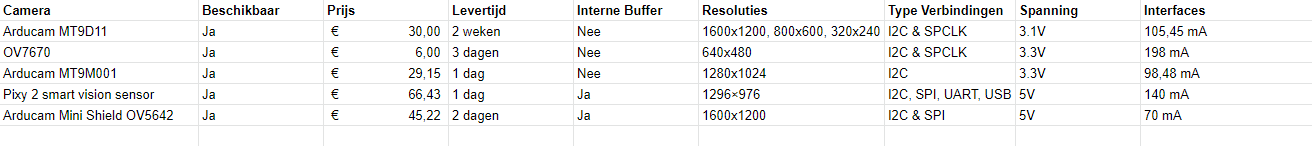
\includegraphics[width=40em]{table2}
	\centering
	\caption{Deelvragen 1 {\&} 2}
	\label{fig:deelvragen1en2}
	\end{figure}

In figure \ref{fig:deelvragen1en2} zie je een tabel met in de linkerkolom de 5 gekozen camera's. In de overige kolommen zie je de eigenschappen en in welke mate de betreffende camera deze eigenschap bezit.

Wij interpreteren de volgende factoren als van belang voor ons onderzoek:
\begin{itemize}
	\item \textbf{Beschikbaar}, is de camera beschikbaar in Nederland?
	\item \textbf{Prijs}, de prijs van de camera. Dit is een belangrijke factor omdat we tijdens de corona crisis maar €28,- per persoon te besteden hebben aan electronica. Daar kunnen we nog wel iets overheen omdat niet alle teamgenoten dat bedrag uitgeven maar we kunnen niet heel ver uitschieten.
	\item \textbf{Levertijd}, de tijd dat het kost tussen bestellen en het in huis hebben. Deze factor is ook vrij belangrijk geworden door de corona crisis. We moeten de camera wel op tijd in huis hebben om het onderzoek af te kunnen ronden en eventueel iets te bouwen.
	\item \textbf{Interne Buffer}, een aanwezig register op de chip om beelden op te bufferen. Deze buffer kan voor ons voordelen opleveren tijdens het coderen. Door een buffer te hebben kan het makkelijker zijn om plaatjes vanaf de camera op de Arduino te zetten. Dan hoeft dit proces namelijk niet hard realtime te gebeuren, maar kan het gebeuren op een moment dat het ons uitkomt.
	\item \textbf{Resolutie}, welke resolutie heeft de camera? De resolutie kunnen we gebruiken om het aantal pixels te berekenen dat 1 plaatje zou bevatten. Daarmee kunnen we dan uitrekenen of het te bufferen is op het RAM geheugen voor we code en testen gaan schrijven.
	\item \textbf{Type Interface},  met welke interface kunnen we de camera verbinden? Het type interface is belangrijk vanwege de verbindingsmogelijkheden. Als de camera gebruik maakt van een interface die niet te gebruiken is icm een Arduino kunnen we de camera helemaal niet gebruiken. Verder is het fijn als er een interface gebruikt wordt waar al code voor bestaat binnen het bedrijf. Hier hoeven we dan geen tijd aan te besteden bij het onderzoek.
	\item \textbf{Spanning}, wat voor spanning heeft de camera nodig? De hoeveelheid benodigd voltage is natuurlijke een belangrijke factor omdat het invloed heeft op verschillende andere factoren. Als de benodigde spanning te hoog ligt voor een Arduino, dan zou de prijs van het totaal weer omhoog gaan omdat we dan met een relais of transistoren moeten gaan schakelen. Daarbij wordt dan de levertijd wellicht beïnvloed. Wanneer de spanning boven de maximum spanning van een Arduino komt (5v) wordt de camera dus minder interessant om te gebruiken. 
	\item \textbf{Stroomverbruik in gebruik}, hoeveel Ampère is het stroomverbruik tijdens gebruik van de camera? Het verbruik is om dezelfde reden als de spanning interessant. Wanneer het stroomverbruik hoger is dan een Arduino zou kunnen leveren ontstaan er problemen bij andere factoren.
\end{itemize}

\subsubsection{Deelvraag 3}
Wij hebben gekozen voor de OV7670. Dit was de enige gevonden camera die binnen ons budget viel. We hadden het budget kunnen vergroten, maar deze camera had ook de laagste resolutie. Dit vergroot de kans dat de afbeelding gebufferd kan worden op de Arduino Due. Daarbij moet de camera ook te koop zijn voor andere groepjes ten tijden van de module wisseling.  Deze camera is ook beschikbaar in de webwinkel van een van onze docenten, Wouter van Ooijen. Zo kunnen we hem altijd om hulp vragen als het nodig is. Gezien de corona crisis is dat laatste voor ons wel belangrijk, hulp op afstand. Verder is de camera te benaderen met een I2C interface en beide onderzoekers hebben hier enige ervaring mee, wat het communiceren met de chip makkelijk maakt. Maar de doorslaggevende factor is uiteindelijk de prijs en de levertijd geweest. Ook met het oog op de eventuele module wisseling.

\subsubsection{Deelvraag 4}
De Arduino Due heeft 96kb ram. De OV7670, onze gekozen camera, maakt een afbeelding met een resolutie van 640x480. Dit zijn 307.200 pixels in het totaal. De module gebruikt 1 byte per pixel als een bayer filter die we moeten decoden. In het totaal is dat dus ongeveer 0,3mb. De Arduino Due heeft volgens de berekening dus niet genoeg geheugen voor het opslaan/bufferen van 1 frame.

Onze oorspronkelijke hypothese voorafgaand aan het onderzoek was dat de Arduino wel voldoende geheugen zou hebben. Daarom was ons oorspronkelijke plan ook om daar dan code voor te schrijven. Nu blijkt natuurlijk al dat dat geen zin heeft maar we willen toch code schrijven en een degelijk onderzoek neerzetten.
Uit heel kort zoekwerk op internet blijkt beperkt geheugen een bekend probleem en er zijn verschillende mensen te vinden die hier \href{vragen}{https://forum.arduino.cc/index.php?topic=159557.0} over stelde. Op Github hebben we uiteindelijk een persoon gevonden die in zijn \href{main}{https://github.com/ComputerNerd/ov7670-simple/blob/master/main.c} dit probleem oplost. Het probleem wordt hier opgelost door het bestand (de foto) in meerdere delen op te delen en hem dan in delen te bufferen op de Arduino. 

Als gevolg daarvan hebben wij besloten onze hypothese aan te passen en aan te nemen dat de Arduino Due niet voldoende geheugen heeft om 1 frame te bufferen.


\subsubsection{Deelvraag 5}
Door het beperkte geheugen op de DUE zijn wij in staat om slechts een deel van een frame te bufferen. Dit deel is XXXX \% van het frame. 

\section{Resultaten}
De onderzoeksvragen, theorie en hypotheses worden hier kort samengevat. Hier volgen nog geen interpretatie wel getalsmatige conclusies.

\section{Conclusie en discussie}
Hier worden de resultaten in verband gebracht met de vraagstelling en worden de conclusies en verbanden gelegd.

\section{Evaluatie}
Hier wordt het onderzoek geëvalueerd op product- en procesniveau. Er wordt dus gekeken naar de sterke en zwakke punten van het onderzoek, de leerervaringen en eventuele zaken die verkeerd zijn gegaan en in de toekomst anders zouden moeten. Verder wordt een onderzoekslogboek bijgevoegd waarin de dagelijkse besluiten en gebeurtenissen in staan.

\section{Aanbevelingen}
Hier kunnen eventuele aanbevelingen worden gedaan op basis van de conclusies en resultaten.

\section{Suggesties voor verder onderzoek}
Mochten er tijdens het onderzoek nieuwe vragen naar voren zijn gekomen of nog onbeantwoorde vragen overgebleven zijn dan kunnen hier suggesties worden aangegeven. Deze kunnen dan eventueel in een nieuwe onderzoek meegenomen worden.

\section{Literatuur}
In de literatuurlijst geef je op alfabetische volgorde aan welke literatuur je tijdens je onderzoek hebt gebruikt. Het is dan ook aan te raden om tijdens je onderzoek goed bij te houden welke bronnen je hebt gebruikt en wat je precies uit die bronnen hebt gehaald.

\section{Bijlagen}
Stukken die niet in je onderzoeksrapport past kan je in de bijlagen plaatsen. Denk hierbij aan vragenlijsten, observatieschema’s, codeerschema’s, brieven aan respondenten, etc.
klein voorbeeld van mensen met vragen over data opslag OV7670

https://forum.arduino.cc/index.php?topic=159557.0
stuk met extra code die probleem data opslag tackelt
https://github.com/ComputerNerd/ov7670-simple/blob/master/main.c

\end{document}